\begin{frame}
\begin{itemize}
	\item Dérivé de Logo
		
\includegraphics[scale=0.4]{doc/Presentation/image/logo.pdf}
	\item Inspiré de NetLogo et de StarLogo
		
\includegraphics[scale=0.3]{doc/Presentation/image/netlogo.pdf}
		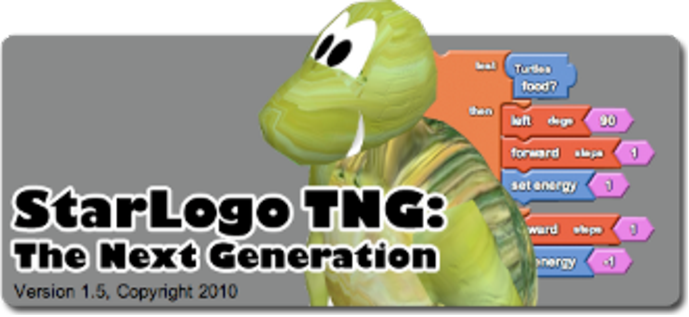
\includegraphics[scale=0.4]{doc/Presentation/image/starlogo.pdf}
\end{itemize}
\end{frame}

\begin{frame}
\frametitle{Le projet Stibbons}
\begin{itemize}
	\item Un langage de programmation multi-agents
	\item Un interprète de ce langage
	\item Un modèle
	\item Une application graphique
\end{itemize}
\end{frame}

\begin{frame}
\frametitle{Le langage Stibbons}
\begin{itemize}
        \item Typage dynamique
        \item Propriétés des agents
        \item Fonctions, boucles, conditionnelles, etc.
        \item Définitions de types d'agents
        \item Nouvel agent = nouveau thread
        \item Communication entre agents mobiles
        \item Bibliothèque standard
\end{itemize}
\end{frame}
